\documentclass[../projekt.tex]{subfiles}
\begin{document}


\chapter{OpenAPI specification 2.0}\label{openapispec}
OpenAPI Specification (OAS) opisuje štandard dokumentácie pre REST API. Vďaka tejto špecifikácii je možné jednotným jazykom dokumentovať rôzne aplikačné rozhrania. Tým pádom mohli vzniknúť nástroje na vytváranie grafických dokumentácií. V~súčasnosti sú populárne napríklad Swagger alebo Apiary.


\begin{figure}[h]
 
\begin{subfigure}
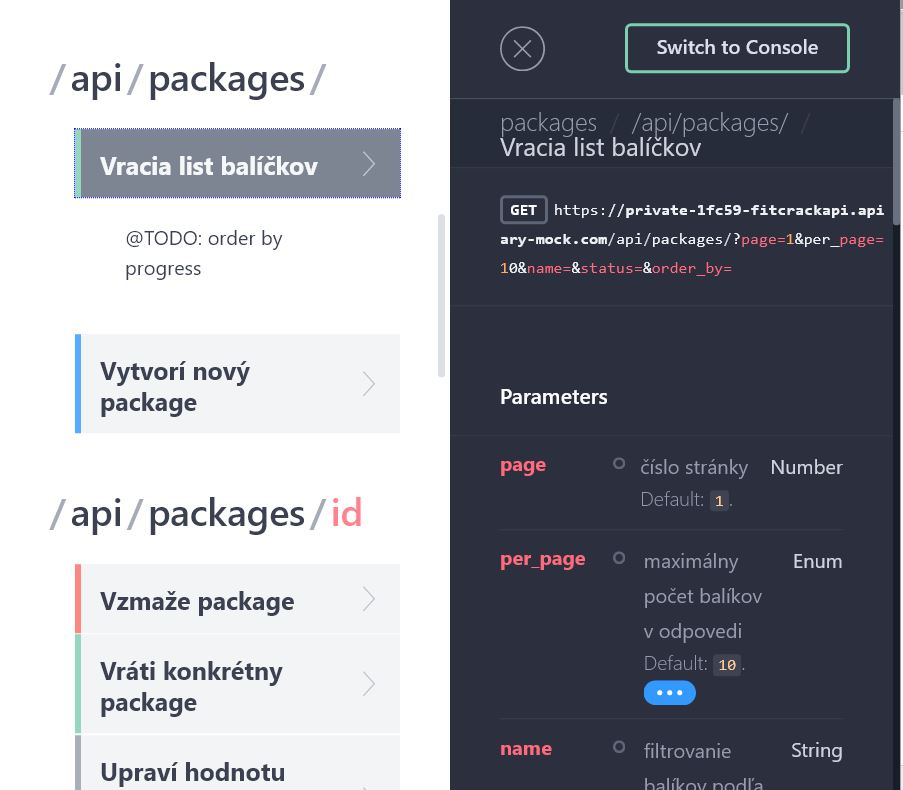
\includegraphics[width=0.5\linewidth, height=6cm]{obrazky/doc1.JPG} 
\label{fig:subim1}
\end{subfigure}
\begin{subfigure}
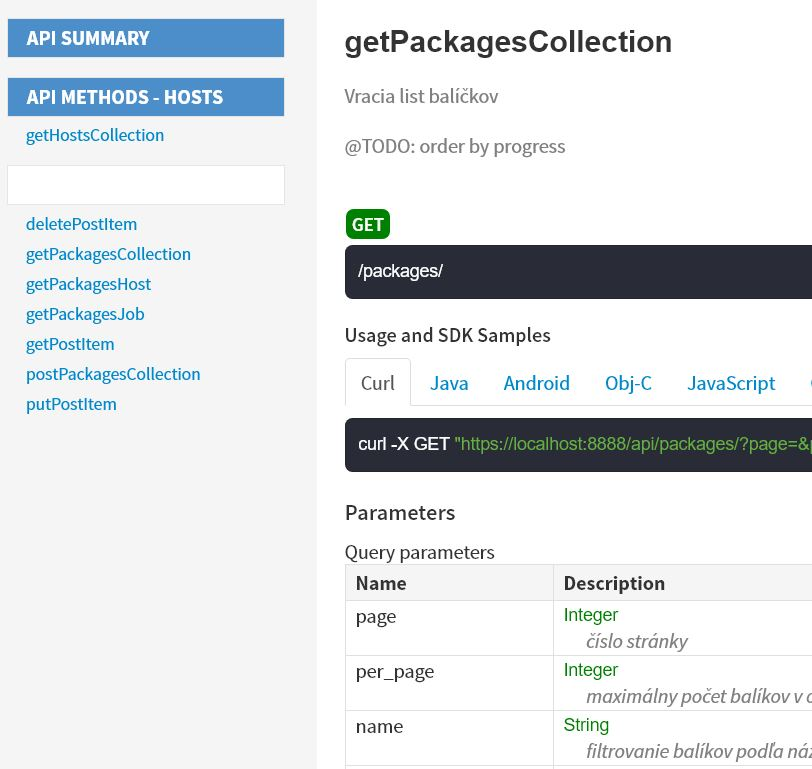
\includegraphics[width=0.5\linewidth, height=6cm]{obrazky/doc2.JPG}
\label{fig:subim2}
\end{subfigure}
 
\caption{Dokumentácie vygenerované rôznymi nástrojmi}
\label{fig:image2}
\end{figure}

\section{Formát}
Najčastejšie je aplikačné rozhranie, opísané pomocou OAS, zapísané pomocou formátu JSON. Taktiež môže byť zapísané vo formáte YAML, keďže YAML je nadmnožinou formátu JSON. Všetky položky v~špecifikácii rozlišujú malé a veľké písmená.

\section{Dátové typy}
V~špecifikácii sú pevne definované dátové typy, ktoré sa v~nej môžu použiť. Sú to \texttt{integer, long, float, double, string, byte, binary, boolean, date, dateTime} a \texttt{password}

\section{Obsah špecifikácie}
Špecifikácie obsahuje hlavičku, v~ktorej sú uvedené informácie názov aplikačného rozhrania, krátky popis, podmienky použitia, kontakt na správcu, licencia a verzia aplikačného rozhrania. Ďalej špecifikáciu API tvoria jednotlivé URI k~zdrojom. Tie obsahujú HTTP metódy cez ktoré sa k~nim pristupuje. Jednotlivé metódy potom obsahujú formáty odpovedí, povinné a voliteľné parametre a popis danej operácie.
\newline


\begin{lstlisting}[caption=Príklad hlavičky OAS,frame=tlrb]{Name}
title: Fitcrack API
description: RESTful api vytvorené pre systém Fitcrack
contact:
  name: Autor Api
  url: www.stud.fit.vutbr.cz/~xmucka03/
  email: xmucka03@stud.fit.vutbr.cz
version: 1.0.1
\end{lstlisting}





\end{document}